% Note: This template was adapted by a report template created by Kartik Singhal under theCreative Commons Attribution 4.0 International License. You can their template at the repository linked [here](https://github.com/googol-lab/latex-project-report-template)
% 
% View README.md for further information

\documentclass[12pt]{report}
\usepackage{amsmath}
\usepackage{amssymb}
\usepackage[pdftex]{graphicx} %for embedding images
\usepackage{url} %for proper url entries
\usepackage{appendix} %for appendix functionality
\usepackage[bookmarks, colorlinks=false, pdfborder={0 0 0}, pdftitle={<pdf title here>}, pdfauthor={<author's name here>}, pdfsubject={<subject here>}, pdfkeywords={<keywords here>}]{hyperref} %for creating links in the pdf version and other additional pdf attributes, no effect on the printed document
%\usepackage[final]{pdfpages} %for embedding another pdf, remove if not required

\usepackage{listings}
\usepackage{color} %red, green, blue, yellow, cyan, magenta, black, white
\definecolor{mygreen}{RGB}{28,172,0} % color values Red, Green, Blue
\definecolor{mylilas}{RGB}{170,55,241}
\usepackage{geometry} % Widen margins for code listings
\newgeometry{left = 1in, right = 1in, top = 1in, bottom = 1in}

% Below is listing settings for MATLAB code
\lstset{language=Matlab,%
    %basicstyle=\color{red},
    basicstyle=\footnotesize\ttfamily,
    breaklines=true,%
    morekeywords={matlab2tikz},
    keywordstyle=\color{blue},%
    morekeywords=[2]{1}, keywordstyle=[2]{\color{black}},
    identifierstyle=\color{black},%
    stringstyle=\color{mylilas},
    commentstyle=\color{mygreen},%
    showstringspaces=false,%without this there will be a symbol in the places where there is a space
    numbers=left,%
    numberstyle={\tiny \color{black}},% size of the numbers
    numbersep=9pt, % this defines how far the numbers are from the text
    emph=[1]{for,end,break},emphstyle=[1]\color{red}, %some words to emphasise
    %emph=[2]{word1,word2}, emphstyle=[2]{style},    
    breaklines=true,
    postbreak=\mbox{\textcolor{red}{$\hookrightarrow$}\space},
}    % Import the listings package & MATLAB style 

\usepackage{titlesec}
\titleformat{\chapter}[block]
  {\normalfont\huge\bfseries}{\thechapter}{20pt}{\Huge} % Formats chapters so number and chapter name are inline, comment out to revert to default  

\begin{document}
\renewcommand\bibname{References} %Renames "Bibliography" to "References" on ref page

%include other pages
\begin{titlepage}

\begin{center}

\textup{\small {\bf <Course code goes here>} \\ <Course name goes here> \\ <Report number/ID goes here>}\\[0.2in]

% Title
\Large \textbf {<Title here>}\\[0.5in]

% Submitted by
\normalsize Submitted by \\
<name goes here>\\

\vspace{.3in}
Instructed by\\
{\textbf{<Instructor's name here>}}\\[0.2in]

\vfill

% Bottom of the page

\includegraphics[width=0.18\textwidth]{./Images/LaTeX_logo.png}\\[0.1in]
\Large{<Department/school name goes here>}\\
\normalsize
\textsc{<Institution name goes here>}\\
<location goes here> \\
\vspace{0.2cm}
<date goes here>

\end{center}

\end{titlepage}

% \vspace{2in}
\begin{abstract}

<Abstract here>

\end{abstract} 


\pagenumbering{roman} %numbering before main content starts
\tableofcontents
\listoffigures

\newpage
\pagenumbering{arabic} %reset numbering to normal for the main content


\chapter{Introduction}

\section{<Section Title>}

\section{<Section Title>}

\subsection{<any sub section here>}
some text\cite{citation-1-name-here}, some more text\footnote{<footnote here>} 
\chapter{Procedures}

\section{<Section title>}

\subsection{<Sub-section title>}

\subsection{<Sub-section title>}

Refer figure \ref{fig:label}.

\begin{figure}[htb]
\centering
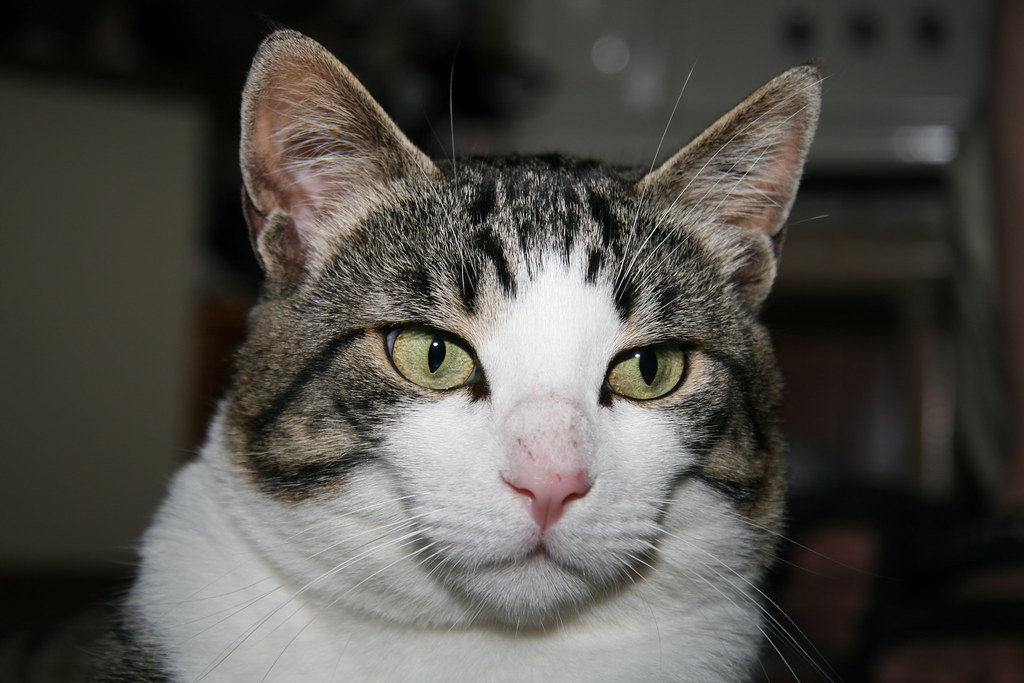
\includegraphics[scale=0.3]{./Images/PlaceholderCat.jpg} % e.g. insert ./image for image.png in the working directory, adjust scale as necessary
\caption{<Caption here>}
\label{fig:label} % insert suitable label, this is used to refer to a fig from within the text as shown above
\end{figure}

\section{<Section title>}


\chapter{Results}

\section{<Section title>}
some text\cite{citation-2-name-here}, some more text

\section{<Conclusion>}
<Conclusion here>
\cleardoublepage
%\pagebreak
\phantomsection
\addcontentsline{toc}{chapter}{References}
\begin{thebibliography}{99}

\bibitem{citation-1-name-here}<Name of the reference here>,\ \url{<url here>}

\bibitem{citation-2-name-here}<Name of the reference here>,\ \url{<url here>}

\end{thebibliography}

\appendix
\appendixpage
\addappheadtotoc

\chapter{<Appendix Name>}

\end{document}
